%
% Latex example file for postgrads (04/10/03)
%
% If you have questions please email me: 
% M.L.Balogh@durham.ac.uk
% or find me in room OC312.
%
% Note you can get Latex style files etc. from http://www.ctan.org


% Use emulateapj instead to make Apj format.
% YOU SHOULD REMOVE THE TABLE OF
% CONTENTS PAGE WHEN USING APJ FORMAT.
\documentclass[11pt,a4paper]{emulateapj}
\bibliographystyle{apj}


%define general packages
\usepackage{epsfig}
\usepackage{amsmath}
\usepackage{natbib}

% spanish packages
\usepackage[utf8]{inputenc}
\usepackage[spanish]{babel}
\languageshorthands{none}
\noextrasspanish
\let\layoutspanish\relax
\usepackage[spanish]{babel}
\renewcommand\shorthandsspanish{}

%internal short cuts
\def \HgA {H$\gamma_A$}
\def \gon {Gonz\'{a}lez}
\def \Hbp {H$\beta ^\prime$}
\def \warn {{\sffamily\bfseries\large WARNING, ARREGLAR:}}









\begin{document}

\submitted{Departamento Ing. en Informática, ITBA}
\title{La cuerda en el iPhone}
\author{Williams M. \& Aráoz M.}
\date{\today}


\begin{abstract}
En la vida cotidiana, se puede observar que muchos objetos se comportan respetando la ecuación de ondas. Esto genera la necesidad de poder simular este comportamiento. Para lograr esta simulación se necesita un modelo númerico que se obtenga de la ecuación misma. En este trabajo se utiliza la ecuación de ondas contemplando una amortiguación para representar el comportamiento de una cuerda. 
\end{abstract}

\maketitle




\section{Introduccción}
\label{sec:introduccion}
La ecuación de ondas se puede utilizar para representar diferentes objetos de la vida cotidiana. La forma más simple de representar la ecuación de ondas es la siguiente:
\begin{equation}
\label{eq:ondas}
\frac{\partial ^2 u}{\partial t^2} = c^2 \nabla ^2 u
\end{equation}
, donde $\nabla ^2$ es el laplaciano y $c$ es una constante que depende del problema. Para poder hacer uso de la ecuación (\ref{eq:ondas}) dentro de un dispositivo de cálculo se debe discretizar la ecuación con el fin de obtener una aproximación que se pueda ingresar al dispositivo. Para lograr esto primero se debe obtener una aproximación de las derivadas parciales y luego se debe discretizar estas aproximaciones. Una vez realizado esto, se obtiene el siguiente método para calcular $u(x,t)$ de forma aproximada a partir de las condiciones de borde del problema $u(0,t) = L_1$ y $u(L,t) = L_2$ teniendo en cuenta que $0 < x < L$ y de la condición inicial $u(x,0) = g(x)$:
\begin{eqnarray}
	\label{eq:metodoDeOndas}
	\left\{
		\begin{matrix}
			u_i^{n+1} = (2-2r) u_i^n + r^2 (u_{i-1}^n+u_{i+1}^n) - u_i^{n-1}\\
			u_j^0 = g(\Delta x\, j)\\
			u_0^n = L_1\\ 
			u_N^n = L_2\\
		\end{matrix} \right.
\end{eqnarray}
, donde $u_i^{n} \approx u(x_j,t^n)$, con $x_j = \Delta x\, j$ y $t^n = \Delta t\, n$.
Este método se utiliza en este trabajo para realizar una simulación del comportamiento de una cuerda en un iPhone, a la cual se le pueden efectuar perturbaciones externas que generan que se mueva siempre respetando la ecuación de ondas.

\section{Amortiguación}
El método planteado en la ecuación (\ref{eq:metodoDeOndas}) genera que la cuerda nunca deje de moverse pues no tiene amortiguación el movimiento. Si se piensa la amortigación como una función que depende de la velocidad con la que se mueva la cuerda, se la puede plantear de la siguiente forma:
\begin{equation}
\label{eq:amort}
-\beta \frac{\partial u}{\partial t}
\end{equation}
Si se agrega la amortiguación de la forma planteada en (\ref{eq:amort}) a la ecuación de ondas (\ref{eq:ondas}), se obtiene la siguiente ecuación:
\begin{equation}
\label{eq:amortImpl}
\frac{\partial ^2 u}{\partial t^2} = c^2 \frac{\partial ^2 u}{\partial x^2} - \beta \frac{\partial u}{\partial t} 
\end{equation}
Una vez planteada la ecuación falta discretizarla para poder llevarla a un dispositivo de cómputo que permita correr la simulación de la cuerda. Para aproximar las derivadas parciales de segundo orden se utilizó la siguiente aproximación:
\begin{equation}
\frac{\partial ^2 u}{\partial t^2}(x,t) = \frac{u(x,t-h) -2 u(x,t) + u(x,t+h)}{h^2} +\vartheta(h^2)
\end{equation}
Por otro lado, para calcular la derivada parcial de primer orden se utilizó una aproximación de orden lineal:
\begin{equation}
\frac{\partial u}{\partial t}(x,t) = \frac{u(x,t) - u(x,t-h)}{h} +\vartheta(h)
\end{equation}
Por último, discretizando las aproximaciones y utilizando la ecuación (\ref{eq:amortImpl}) se puede plantear un método discreto que considere la amortiguación:
\begin{eqnarray}
	\label{eq:metodoDeOndas}
	\left\{
		\begin{matrix}
			u_i^{n+1} = (2-2r) u_i^n + r^2 (u_{i-1}^n+u_{i+1}^n) - u_i^{n-1} - \beta\Delta t(u_i^n - u_i^{j-1})\\
			u_j^0 = g(\Delta x\, j)\\
			u_0^n = L_1\\ 
			u_N^n = L_2\\
		\end{matrix} \right.
\end{eqnarray}	
, donde $r = \dfrac{\Delta t}{\Delta x}c$.

\section{Implementación en el iPhone}
Para implementar el algoritmo en el iPhone se tomaron algunas decisiones respecto de los parámetros computacionales:
\begin{enumerate}
	\item Se fijó $r$ de manera que el método sea estable, en vez de definir $\Delta x$ y $\Delta t$ tal que $r$ sea estable. Es posible realizar esto, porque al ser una animación los intervalos no modifican el resultado. Es decir, se pueden ver más cuadrados o no las puntas de la cuerda definiendo $\Delta x$ pero no modifica el resultado que se busca obtener con la simulación.
	\item No se guardan todos los tiempos de la discretización de la función $u(x,t)$, ya que no son necesarios para la animación. Solo se utilizan los dos tiempos anteriores, entonces con esos datos alcanza en todo momento para calcular la nueva posición de cada punto de la cuerda.
\end{enumerate}
\section{Resultados y Conclusiones}
\label{sec:resultadosyconclusiones}

Como resultados de este trabajo, se obtuvieron las simulaciones para los dos métodos (con amortiguación y sin amortiguación). En el caso del modelo con amortiguación, la cuerda se comportó como se esperaría que lo hiciera en el mundo real, mientras que cuando el modelo no contemplaba amortigución esto no sucedía pues nunca dejaba de moverse.  
\begin{figure}[ht!]
     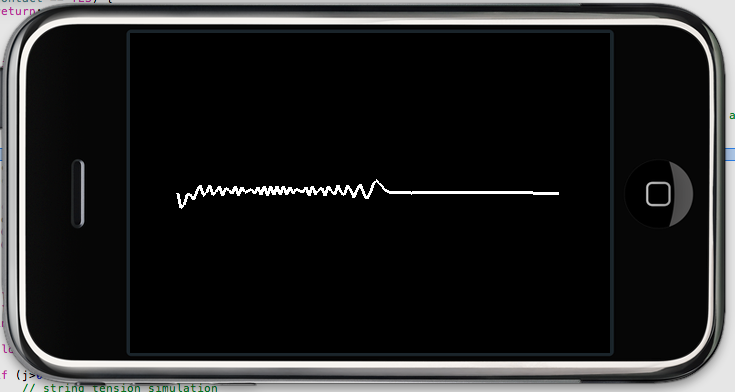
\includegraphics[width=120px]{images/amortInit.png}
      \caption{cuerda respetando el modelo amortiguado en el simulador de iPhone, en el instante inicial.}
     \label{fig:amortInit}
\end{figure} 
\begin{figure}[ht!]
     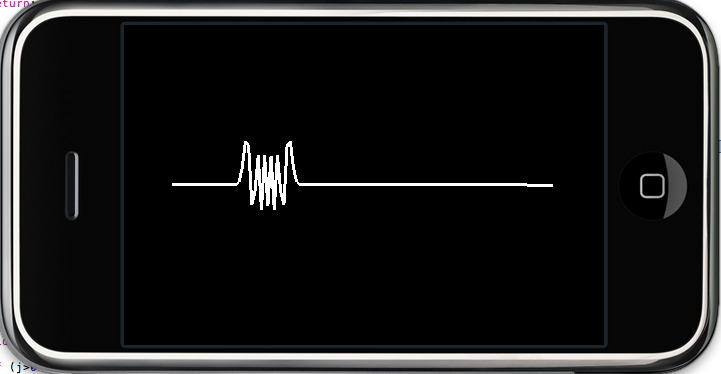
\includegraphics[width=120px]{images/amortFinal.png}
      \caption{cuerda respetando el modelo amortiguado en el simulador de iPhone, en el instante final.}
     \label{fig:amortFinal}
\end{figure}
 
Para mostrar la simulación se tomaron dos tiempos, el inicial y uno final. En la figura (\ref{fig:amortInit}) se puede ver la simulación de la cuerda utilizando el modelo amortiguado en el momento inicial mientras que en la figura (\ref{fig:amortFinal}) se puede ver la misma simulación luego de una determinada cantidad de tiempo.

\begin{figure}[ht!]
     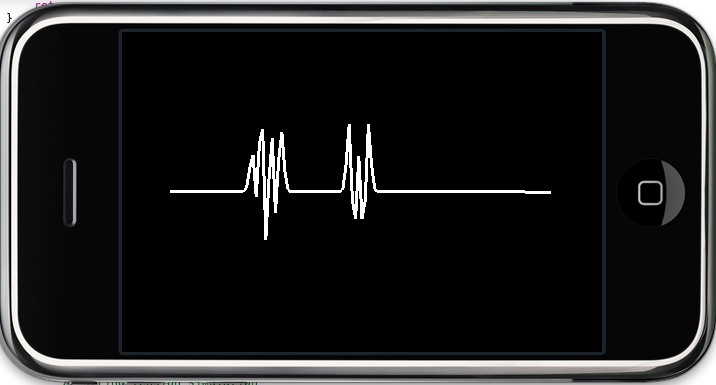
\includegraphics[width=120px]{images/sinamortInit.png}
      \caption{cuerda respetando el modelo no amortiguado en el simulador de iPhone en el instante inicial.}
     \label{fig:sinamortInit}
\end{figure}
\begin{figure}[ht!]
     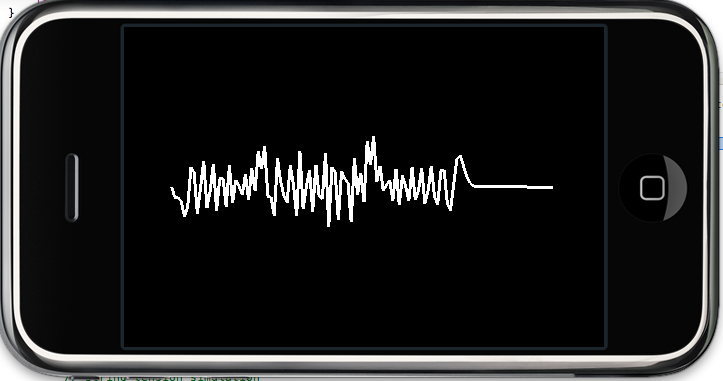
\includegraphics[width=120px]{images/sinamortFinal.png}
      \caption{cuerda respetando el modelo no amortiguado en el simulador de iPhone en el instante final.}
     \label{fig:sinamortFinal}
\end{figure}

Utilizando los mismos tiempo para el modelo amortiguado se obtienen la figura la figura (\ref{fig:sinamortInit}) en el momento inicial y la figura (\ref{fig:sinamortFinal}) en el instante final.  Para ambos casos se ha utilizado la misma pertubación inicial.
 

%
% References
%
\bibliography{paper}

\end{document}

